\documentclass{manual}

\title{ANUGA Installation Guide}

\usepackage{graphicx}
\usepackage{hyperref}

% Please at least include a long-lived email address;
% the rest is at your discretion.
\authoraddress{Geoscience Australia \\
  Email: \email{anuga@ga.gov.au}
}

%Draft date
\date{\today}                   % update before release!
                % Use an explicit date so that reformatting
                % doesn't cause a new date to be used.  Setting
                % the date to \today can be used during draft
                % stages to make it easier to handle versions.

		
%
% This file is a dummy used if update_anuga_user_manual.py hasn't 
% generated one.
%	
	

% release version; this is used to define the
% \version macro
\release{1.2.1}
 % Get version info - this file may be modified by
                % update_anuga_user_manual.py - if not a dummy 
		% will be used.
				

\makeindex          % tell \index to actually write the .idx file
%\makemodindex          % If this contains a lot of module sections.



\begin{document}
\maketitle



% This makes the contents more accessible from the front page of the HTML.
\ifhtml
\chapter*{Front Matter\label{front}}
\fi




\chapter{Introduction}

This document outlines the procedure for installing the Anuga toolbox.
All components are licensed as open source and readily available from the net.
It is assumed that the reader is familiar with the Python programming language
and the process of downloading, installing and unpacking files into directories.


\section{System requirements}
\label{sec:requirements}

To run ANUGA you will need a Windows PC or a Linux PC with at 
least 1GB RAM.  As ANUGA is a memory-intensive numerical system, more memory is better than less.

The viewer (Windows only) requires a graphics adapter that
is OpenGL compatible. It has been tested with ATI FireGL X1 cards
and the NVIDIA family. It may not work with other cards such as those from the
Intel(R) 82915G Express chipset family.

We recommend that you check out the page \url{http://anuga.anu.edu.au} for the latest information on installing Anuga. 

%Where the text below refers to a specific package file such as \code{python-2.5.msi} you will find that
%file in a download area linked through the \emph{numpy_support_software} link on the page
%\url{https://datamining.anu.edu.au/anuga/wiki/NumpyInstall}.


\section{Installation}

Below are the install procedures for Windows 7 (32 bit) and Linux (32 and 64 bit).

\subsection{Install - Windows (32 bit)}
\label{sec:win}



We use PYTHON as our programming environment together with a number of standard PYTHON packages such as numpy, scipy, matplotlib, netcdf4. One way to install all the required packages is to use a distribution like python_xy.

\subsubsection{PYTHON xy}

So first install  python xy. This will be a large download, maybe 500 MB or more, but will provide a complete installation (well see NetCDF4 note below) of python for our needs . You should first remove any other version of python and mingw that may be on your system. The python xy package is currently only 32 bits, but this will still work on 64 bit Windows.

Be sure to choose the win32 python 2.7 version. This is the version for which we are developing.
Netcdf4 Note

Check that netcdf is available. From a command line, try
\begin{verbatim}
python -c "import netCDF4"
\end{verbatim}
If no error occurs then netCDF4 is available and you can disregard the rest of this note.

But unfortunately version 2.7.3.1 (April 2013) python xy seems to be missing netCDF4. Please let us know if later versions are ok.
If it is missing then you need to install another package to cover this loss. For this we can use the precompiled scientific python binaries from  \url{http://www.lfd.uci.edu/~gohlke/pythonlibs/#scientificpython}. I suggest you choose ScientificPython-2.9.2.win32-py2.7.‌exe to install. To test this install try:
\begin{verbatim}
python -c "import Scientific.IO.NetCDF"
\end{verbatim}

\subsubsection{64 bit}

At the moment python xy is only 32 bit, but there seems to be a promise that a 64 bit distribution is not too far away. There is a 64 bit python distribution package from Enthought, but is free only to academic users. So at present we recommend win32 python xy.
Manual install

It is possible to install the required environment manually. You would need to install Mingw to provide a compiler, the standard distribution of python27 and then precompiled python libraries for numpy, scipy, matplotlib, netcdf4 from a site like  \url{http://www.lfd.uci.edu/~gohlke/pythonlibs/}. It would be interesting to hear feedback on this option, as there is an opportunity to use versions using the Intel Math Kernel Library, which should provide a useful increase in speed.
Installing anuga

\subsection{Obtaining ANUGA source}

You can either use the source code avialble from sourceforge or  download the latest version of the package using subversion. 

You can obtain version 1.3 of the package from sourceforge by downloading the file \url{http://sourceforge/p/anuga}


\subsection{Source from development repository}
An alternative is checking out the most recent version of the package using subversion. 

You need a subversion client. I suggest installing  tortoise_svn downloads and then checking out the following svn repository. When you installed tortoise svn it creates a few extra menu items to your right click menu in the file manager. Just choose "tortoise" checkout to download the code.
\begin{verbatim}
https://anuga.anu.edu.au/svn/anuga/trunk/anuga_core
\end{verbatim}
This should produce an anuga_core directory



\subsection{Setup PYTHONPATH}

We need to tell python where the anuga source code is located. This is done via the PYTHONPATH environment variable.

For instance, if your anuga_core directory was located at

\begin{verbatim}
C:\Users\Steve\anuga_core
\end{verbatim}

then you should add

\begin{verbatim}
C:\Users\Steve\anuga_core\source
\end{verbatim}

to your PYTHONPATH

Environment variables are accessed via control panel -> advanced system settings -> Environment Variables and then add a new Environment variable PYTHONPATH with value \verb|C:\Users\Steve\anuga_core\source| (or what ever is appropriate for your installation)

\subsection{Compiling ANUGA}

Now go to the directory anuga_core and compile the anuga files. Fire up a cmd terminal, change to the anuga_core directory and run
\begin{verbatim}
python compile_all.py
\end{verbatim}
Check that all the files have been compiled correctly. There should be an "OK" at the end of each separate compile command.

\subsection{Run Unit tests}

From the anuga_core directory run the unit tests via:
\begin{verbatim}
python test_all.py
\end{verbatim}

\subsection{Conclusion}

Hopefully all the unit tests pass. As this is bleeding edge there are sometimes a small number of failures as this is a work in progress. Have a look at the demos in the directory anuga_core/documentation/user_manual/demos (along with the user manual) to see how to use anuga.
Updating

\subsection{Updating}
If you downloaded  the source using subversoin, you can update your version of ANUGA. 
 This is fairly easy. Just choose the directory to "update" and then right click and choose "tortoise update" to update the code.

Then again from the anuga_core directory recompile the code and check the unit tests via

python compile_all.py
python test_all.py




%If you already have previous versions of Python, ANUGA support software or the ANUGA source code installed 
%on the target machine, start off by uninstalling them. Next, download the latest version of the ANUGA 
%Windows installer from \url{http://sourceforge.net/projects/anuga/files/}. The Windows installer will 
%install Python, MingW (select the "Minimal" install), NumPy, NetCDF, Scientific Python, Matplotlib, the 
%ANUGA source code and the viewer (animate). Note that you will need an internet connection to install MingW.
%
%After all the necessary packages have been installed, the installer will proceed to compile the ANUGA C code, 
%run the test suite (optional) and then run a series of validation examples (optional). This may take some time.
%Try the demonstrations provided in the ANUGA directory \code{anuga\_demos} (discussed in the ANUGA user manual at 
%\url{https://datamining.anu.edu.au/anuga/attachment/wiki/WikiStart/anuga_user_manual-1.2.0.pdf}) 
%and view the resulting \code{.sww} files with the ANUGA viewer.



%To run the ANUGA against the Okushiri Island wave tank validation dataset
%(\url{http://www.cee.cornell.edu/longwave})
%go to \code{anuga_validation}
% into
%any directory and run the scripts \code{create_okushiri.py},
%\code{run_okushiri.py} and \code{compare_timeseries.py}.  See also the
%\code{README.txt} file that comes with the validation scripts for more
%details.

\subsection{Quick install - Windows Vista and 7}
\label{sec:winvista}

The installation of the support software and the ANUGA software should be the same as for Windows XP above.
The installation and use of ANUGA under Windows Vista and 7 have not been heavily tested.  Feedback on any aspect
of using ANUGA under Vista or 7 is welcomed.

\subsection{Quick install - Linux}
\label{sec:linux}

Please note that the following applies only to Ubuntu 10.04 (\"Lucid Lynx\"). We currently do not
support any other Linux distributions.

\subsubsection{Method 1}

Choose the appropriate deb package for your architecture, download and use the package installer to install.

i386: \url{https://sourceforge.net/projects/anuga/files/anuga_ubuntu_package/python-anuga_1.2.0-0ubuntu3_i386.deb/download}\\
AMD64: \url{https://sourceforge.net/projects/anuga/files/anuga_ubuntu_package/python-anuga_1.2.0-0ubuntu3_amd64.deb/download}

\subsubsection{Method 2}

Open a terminal and enter:
\begin{verbatim}
sudo add-apt-repository ppa:anuga/ppa
sudo apt-get update
sudo apt-get install python-anuga
\end{verbatim}

\subsubsection{Method 3}

Add the following lines to your \code{/etc/apt/sources.list}:
\begin{verbatim}
deb http://ppa.launchpad.net/anuga/ppa/ubuntu lucid main
deb-src http://ppa.launchpad.net/anuga/ppa/ubuntu lucid main
\end{verbatim}
Download the ANUGA key from \url{https://datamining.anu.edu.au/anuga/raw-attachment/wiki/WikiStart/anuga.key}. You can add this key with:
\begin{verbatim}
sudo apt-key add anuga.key
\end{verbatim}
or go to System -$>$ Administration -$>$ Software Sources -$>$ Authentication -$>$ Import Key File

Open a terminal and enter:
\begin{verbatim}
sudo apt-get update
sudo apt-get install python-anuga
\end{verbatim}




\section{Optional but recommended software}
This software is not required to run the ANUGA toolbox, but it is recommended.
\begin{itemize}
  \item psyco. Speeds up ANUGA by about 30\%, so is strongly recommended.
    Under Ubuntu install either through Synaptic or by:
    \begin{verbatim}sudo apt-get install python-psyco\end{verbatim}
    Under Windows install the file \code{psyco-1.6.win32-py25.exe}
    which you can find on the \url{http://psyco.sourceforge.net/download.html} page.

  \item VTK. The Visualization Toolkit. Under Ubuntu install either through Synaptic or by:
    \begin{verbatim}sudo apt-get install python-vtk\end{verbatim}
    Under Windows install the file \code{vtk-5.4.2-win32.exe}
    from the \url{http://www.vtk.org/VTK/resources/software.html} page.
\end{itemize}



\section{Testing}

In the ANUGA root directory, run the test suite:
\begin{verbatim}
python test_all.py
\end{verbatim}
ANUGA has been succesfully installed if the tests pass as follows:
\begin{verbatim}
  ...
  test_data_manager.py
  test_interpolate_sww.py
  test_mesh.py
  test_mesh_interface.py
  test_triangmodule.py
  test_triangmoduleII.py
  test_advection.py
.................................................................................
.................................................................................
.................................................................................
.................................................................................
.................................................................................
.................................................................................
.................................................................................
..........................
----------------------------------------------------------------------
Ran 593 tests in 42.712s

OK
\end{verbatim}

Note that if psycho is not installed, a number of psycho related warnings will appear. These warnings 
can be ignored.

%\section{Other stuff to be included}
%
%\begin{verbatim}
%Install tortoise from downloads (ITs didn't integrate wih explorer).
%In settings set proxy to proxy.agso.gov.au  8080
%%
%
%Install swollen from latest distro (in subversion)
%
%
%\end{verbatim}


\appendix
\chapter{Miscellaneous procedures}
\section{Setting the PATH on Windows}
\label{sec:setwindowspath}

The Windows one-click installer should automatically set the necessary PATH 
environment "System variables". However, in case you do not have
permission to modify the system variable, then the method of setting the PATH environment "User variable" 
for Windows XP is shown here. Setting the variable for Windows Vista should be similar.

\setlength\fboxsep{0pt}
\setlength\fboxrule{1.0pt}

First, open the Control Panel:
\begin{figure}[ht]
  \centerline{\fbox{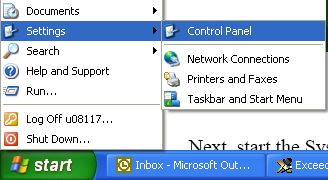
\includegraphics[scale=0.75]{installgraphics/winsetpath1.png}}}
%  \caption{Run Control Panel from the Start menu}
  \label{fig:winsetpath1}
\end{figure}

Next, start the System applet:
\begin{figure}[ht]
  \centerline{\fbox{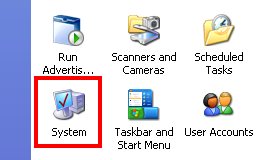
\includegraphics[scale=0.75]{installgraphics/winsetpath2.png}}}
%  \caption{Start the System applet}
  \label{fig:winsetpath2}
\end{figure}

\pagebreak

Select the \code{Advanced} tab in the System Properties window:
\begin{figure}[ht]
  \centerline{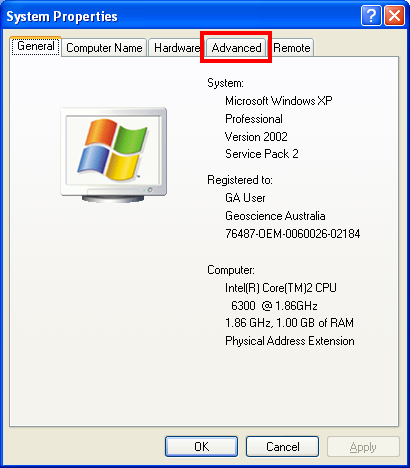
\includegraphics[scale=0.5]{installgraphics/winsetpath3.png}}
%  \caption{Select the Advanced tab}
  \label{fig:winsetpath3}
\end{figure}

%\pagebreak

Press the \code{Environment Variables} button in the \code{Advanced} tab:
\begin{figure}[ht]
  \centerline{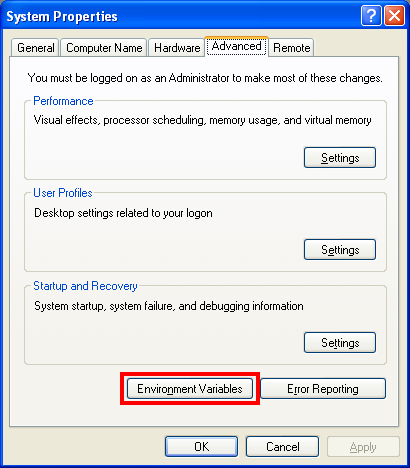
\includegraphics[scale=0.5]{installgraphics/winsetpath4.png}}
%  \caption{Press the Environment Variables button}
  \label{fig:winsetpath4}
\end{figure}

\pagebreak

If the \code{PATH} variable is not defined in the 'User variables' or 'System variables' windows,
press the \code{New} button in either of the two windows (for a personal machine, choose the 'System variables' window).

If \code{PATH} already exists in the 'User variable' or 'System variables' window,
select the row with the \code{PATH} variable name in the appropriate window
and press the \code{Edit} button next to the \code{New} button in that window:
\begin{figure}[ht]
  \centerline{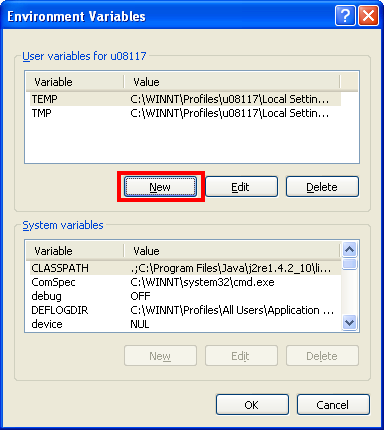
\includegraphics[scale=0.5]{installgraphics/winsetpath5.png}}
%  \caption{Press the New button}
  \label{fig:winsetpath5}
\end{figure}

%\pagebreak

You will be shown the editor window whichever button you pressed in the above step. If the \code{Variable name} box is empty
type in the name \code{PATH}.  In the \code{Variable value} box type the value you want the \code{PATH} variable to have.  If there
is already some text in the box, place your additional value at the front of the existing value, not forgetting to terminate your additional
string with the ';' character. The final value string must be a series of directory names seperated by ';' characters:
\begin{figure}[ht]
  \centerline{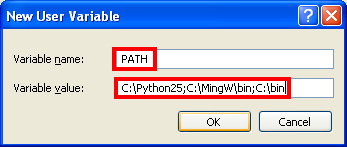
\includegraphics[scale=0.75]{installgraphics/winsetpath6.png}}
%  \caption{Modifying the PATH value}
  \label{fig:winsetpath6}
\end{figure}

When you are finished, press the \code{OK} button and exit from the applet.

\pagebreak

\section{Associating animate.exe with a .sww file}
\label{sec:assocanimatesww}

The one-click installer should associate animate.exe with .sww files automatically. However, the method of associating 
\code{animate.exe} with a \code{.sww} file manually is shown here for Windows XP.
A similar process should work for Windows Vista.

Double left-click on any \code{.sww} file.  This brings up a dialog because Windows doesn't know how to open the file:
\begin{figure}[ht]
  \centerline{\fbox{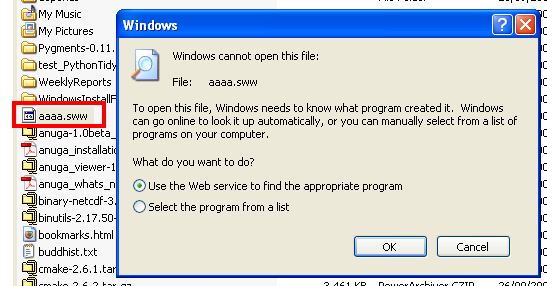
\includegraphics[scale=0.5]{installgraphics/winassoc1.png}}}
%  \caption{Try to open the .sww file}
  \label{fig:winassoc1}
\end{figure}

Select the "\code{Select the program from a list}" radiobutton and press the \code{OK} button:
\begin{figure}[ht]
  \centerline{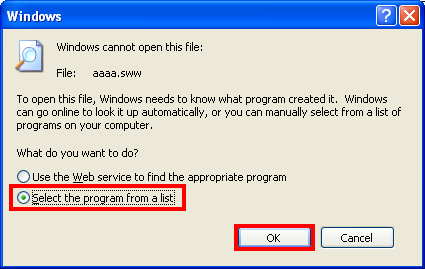
\includegraphics[scale=0.5]{installgraphics/winassoc2.png}}
%  \caption{Select the program from a list}
  \label{fig:winassoc2}
\end{figure}

\pagebreak

Press the \code{Browse...} button to find the \code{animate.exe} program:
\begin{figure}[ht]
  \centerline{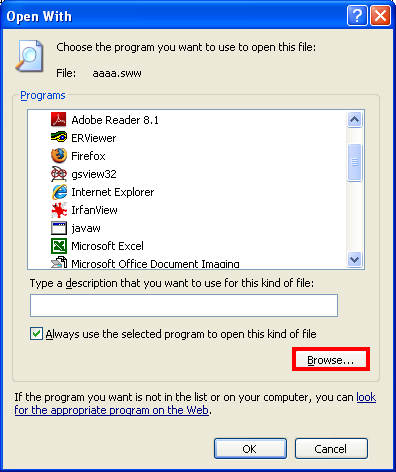
\includegraphics[scale=0.5]{installgraphics/winassoc3.png}}
%  \caption{Find animate.exe program}
  \label{fig:winassoc3}
\end{figure}

Navigate to the \code{C:$\backslash$Program Files$\backslash$anuga_viewer} directory:
\begin{figure}[ht]
  \centerline{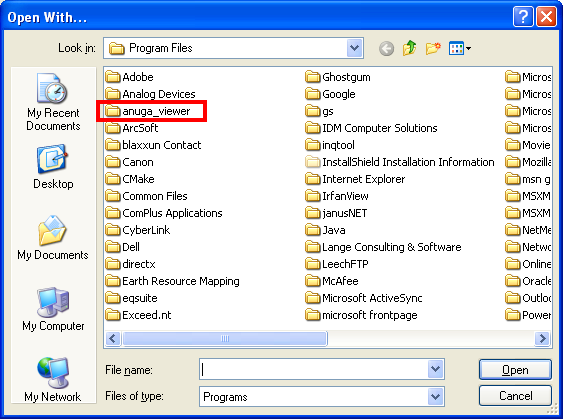
\includegraphics[scale=0.5]{installgraphics/winassoc4.png}}
%  \caption{Navigate into Program Files|anuga_viewer directory}
  \label{fig:winassoc4}
\end{figure}

\pagebreak

Select \code{animate.exe} and press the \code{Open} button:
\begin{figure}[ht]
  \centerline{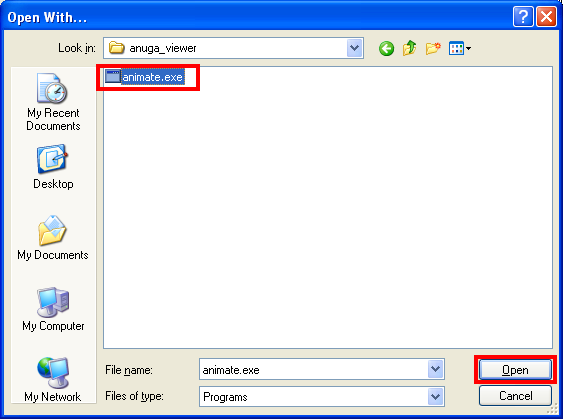
\includegraphics[scale=0.5]{installgraphics/winassoc5.png}}
%  \caption{Select the animate.exe program press Open}
  \label{fig:winassoc5}
\end{figure}

Finally, press the \code{OK} button:
\begin{figure}[ht]
  \centerline{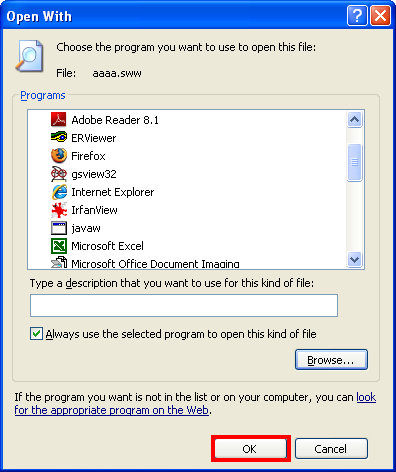
\includegraphics[scale=0.5]{installgraphics/winassoc6.png}}
%  \caption{Press the OK button}
  \label{fig:winassoc6}
\end{figure}


\end{document}
